\documentclass[10pt]{article}
\usepackage[a4paper,margin=1.65cm]{geometry}
\usepackage[T1]{fontenc}
\usepackage[english,french]{babel}
\frenchsetup{SmallCapsFigTabCaptions=false}
\addto\captionsfrench{\renewcommand{\tablename}{Tableau}}
\usepackage{lmodern}
\usepackage{microtype}
\usepackage{graphicx}
\usepackage{booktabs}
\usepackage{tabularx}
\usepackage{array}
\usepackage{amsmath,amssymb}
\usepackage{xcolor}
\usepackage[hidelinks]{hyperref}
\usepackage{caption}
\captionsetup{font=small,labelfont=bf}
\setlength{\parskip}{3.5pt}
\graphicspath{{../research/study09/figures/}}
\newcolumntype{L}[1]{>{\raggedright\arraybackslash}p{#1}}
\newcolumntype{Y}{>{\raggedright\arraybackslash}X}

\title{L'EEG précoce anticipe-t-il la réponse autonome future du stress aigu au-delà du passé physiologique ?\\
\large Audit méthodologique, prévision causale, adaptation LoRA, factorisation trait/état et oculométrie sur 314 personnes (Étude 09)}
\author{Équipe 12 : Mathias Chebbah, Aurélien Saint-Grégoire, Ashley Russo\\
\small HABS Neuro-AI Hackathon, Université Paris-Saclay, novembre 2026}
\date{}

\begin{document}
\maketitle

\begin{abstract}
\noindent Lors d'une exposition brève à un stimulus potentiellement stressant, l'activité électroencéphalographique (EEG) précoce ($[0 ; 5)$~s) apporte-t-elle une information prédictive supplémentaire, spécifique à l'individu et indépendante des artefacts comme du stimulus, sur la réponse autonome future liée au stress ($[5 ; 10)$~s : décélération cardiaque, réactivité électrodermale, respiration), au-delà de ce que la physiologie périphérique précoce ($\text{Corps}[0 ; 5)$~s) prédit déjà ? Nous répondons à cette question sur le jeu de données HABS (314 adultes sains, 22\,974 essais, 252 clips audiovisuels de 10~s) à l'issue d'un protocole pré-enregistré avant calcul (\texttt{journal/09\_eeg\_predictive\_physiology.md}), exécuté exclusivement dans l'ensemble de développement (\texttt{dev}, 12\,693 essais, 228 sujets, 66 thèmes) par validation croisée imbriquée bloquée sujets~$\times$~thèmes avec prétraitements isolés par pli (1,40~H100-h et 3,41~CPU-h). Le split \texttt{test\_new\_both} de l'Étude~08 est traité comme exposé et n'intervient dans aucune validation.

Six résultats principaux émergent. Premièrement, l'audit des Études~07--08 révèle deux biais quantitatifs majeurs que nous corrigeons : le centrage global transductif par sujet (\texttt{person\_center\_matrix}) gonflait la régression logistique de stress sur \texttt{dev} de $+0{,}0141$ (AUC $0{,}5564 \to 0{,}5705$), et le passage bidirectionnel de \texttt{REVE-base} sur $[-3 ; +10)$~s couplé à 77\,\% de thèmes déjà vus gonflait la prévision \texttt{M1} ($\text{EEG}\to\text{Corps}$) de $+0{,}059$ sur le cœur, $+0{,}042$ sur la peau et $+0{,}069$ sur la respiration. Deuxièmement, sous mur causal strict vérifié bit-à-bit à $t = 5{,}000$~s en \emph{cold-start} (Protocole~A), l'EEG précoce (\texttt{REVE-base} gelé) ajoute au passé corporel (\texttt{M0}, $r = 0{,}6849$) un gain prédictif cardiaque \textbf{authentique mais modeste} : $\Delta r = +0{,}0089$ [$+0{,}0054 ; +0{,}0125$] en résiduel ($\Delta R^2_{\text{intra}} = +0{,}0106$, 67,0\,\% des 224 sujets améliorés, $q_{\text{FDR}} < 10^{-6}$), $+0{,}0110$ [$+0{,}0065 ; +0{,}0156$] en Ridge conjoint à double pénalité (71,4\,\% améliorés), $+0{,}0120$ en CV~$5\times 5$, $+0{,}0063$ [$+0{,}0021 ; +0{,}0102$] au-dessus de \texttt{M0\_gbdt} non linéaire, et $+0{,}0182$ [$+0{,}0086 ; +0{,}0276$] sur l'incrément pur $\Delta\mathrm{FC}_{[5;10)-[0;5)}$. Ce gain persiste après bande de garde de 2~s ($[7 ; 10)$~s : $+0{,}0089$) et 5~s ($[10 ; 12)$~s : $+0{,}0038$), résiste à 9 covariables d'artefacts ($+0{,}0085$), aux 46 électrodes intérieures sans bordure ($+0{,}0070$), au contrôle oculométrique ($+0{,}0088$) et à l'essai précédent ($+0{,}0073$), se renforce sur essais propres ($+0{,}0110$), s'annule en permutation intra-sujet ($-0{,}0003$) et sur le pré-stimulus seul ($-0{,}0010$), disparaît après permutation chronologique 1~s, et est \textbf{strictement idiosyncrasique} (remplacer l'EEG par celui d'un autre spectateur devant la même vidéo fait chuter le score de $-0{,}0153$ ; contraste réel contre autre spectateur $+0{,}0242$ [79,0\,\%] ; gain intra-vidéo $+0{,}0065$ [$+0{,}0039 ; +0{,}0091$]). Troisièmement, la même hypothèse est \textbf{réfutée sur la conductance cutanée} ($\Delta r = -0{,}0097$ ; GBDT $-0{,}0155$) et sur la \textbf{respiration} ($\Delta r = +0{,}0008$, tandis que \texttt{M0\_gbdt} seul atteint $0{,}7036$ contre $0{,}6417$ en linéaire et \texttt{M2\_gbdt} vaut $-0{,}0008$, $p = 0{,}453$). Quatrièmement, l'adaptation légère LoRA de \texttt{REVE-base} n'apporte aucun gain par rapport à la représentation gelée (ni en prévision cardiaque $-0{,}0001$, ni en multitâche stress+valence+arousal+ranking $-0{,}0069$ pour 21,7$\times$ plus de temps GPU), alors que la perte de \textbf{ranking intra-sujet} est décisive ($+0{,}0406$ [$+0{,}0266 ; +0{,}0544$] face à son ablation \texttt{norank} qui chute à $0{,}5089$). Cinquièmement, la résidualisation d'état par \emph{shrinkage} bayésien empirique préserve l'AUC intra-sujet ($0{,}5605$ vs $0{,}5609$, battant la soustraction aveugle $0{,}5551$), abaisse la variance d'identité sujet de 51,0\,\% à 36,9\,\% et améliore la calibration globale (AUC poolée $0{,}5302 \to 0{,}5425$, Brier $0{,}2489 \to 0{,}2479$), sans que le sous-espace trait EEG ne prédise la sensibilité-trait subjective ($\rho = -0{,}113$). Sixièmement, l'audit oculométrique des 508 enregistrements confirme une couverture de 96,5\,\% et une corrélation binoculaire de $0{,}852$ avec un décrochage de vitesse du regard à $t = 0{,}00$~s ($+121$~px/s), mais échoue à la porte pupillaire moyenne stricte et reste au hasard en détection de stress ($0{,}5058$) ; enfin, le stacking OOF imbriqué échoue sur toutes les tâches (abstention EDA ; stress $-0{,}0084$, ECG $-0{,}0011$, respiration $-0{,}0057$). Ces résultats établissent une prédiction temporelle incrémentale cerveau--cœur fine et robuste sans revendiquer de causalité mécanistique ni de plafond physiologique.
\end{abstract}

\section{Problématique scientifique autour du stress aigu}

Nos travaux précédents sur le jeu de données HABS (Études~04 à~08) ont caractérisé la cinétique multimodale du stress aigu bref devant des clips audiovisuels de 10~s : les variations corticales EEG apparaissent dès 0--1~s, suivies du freinage vagal cardiaque (allongement de l'intervalle RR sans variation du segment PR) et de la respiration superficielle vers 1--2~s, puis de la réponse électrodermale sympathique vers 4--10~s \cite{palomba2000,hagenaars2014,benedek2010}. Dans l'Étude~08, l'extraction de représentations issues de modèles fondation EEG pré-entraînés (dont \texttt{REVE-base}, 69,2~M paramètres, pré-entraîné sur 60\,000~h) semblait montrer une forte prévision inter-modale $\text{EEG}[0 ; 5)\text{~s} \to \text{Corps}[5 ; 10)\text{~s}$ ($r = +0{,}255$ sur la fréquence cardiaque, $+0{,}136$ sur la conductance cutanée, $+0{,}213$ sur la respiration), sans toutefois améliorer la détection de stress subjectif par rapport aux modèles linéaires de l'Étude~07 \cite{varoquaux2018}.

Avant d'interpréter ce résultat comme une preuve de prédiction cerveau--corps, un audit rigoureux s'imposait. En effet, trois pièges méthodologiques fréquents en neuro-IA affectent ce type de benchmark : (i)~l'utilisation d'un encodeur Transformer \emph{bidirectionnel} sur une fenêtre englobant le futur, qui fait fuiter l'EEG contemporain $[5 ; 10)$~s dans les représentations dites « précoces » $[0 ; 5)$~s ; (ii)~l'absence de comparaison à un modèle autorégressif du passé physiologique seul (\texttt{M0} : $\text{Corps}[0 ; 5) \to \text{Corps}[5 ; 10)$), sans lequel il est impossible de savoir si l'EEG ajoute une information nouvelle ou reflète simplement un état déjà mesurable en périphérie ; et (iii)~la normalisation transductive par participant (\texttt{person\_center\_matrix}) et le partage de thèmes vidéo entre entraînement et évaluation \cite{giannakakis2015,gerster2026}.

L'Étude~09 abandonne donc la recherche d'une maximisation artificielle de l'AUC de stress pour répondre à une question scientifique centrale et à trois déclinaisons pré-enregistrées :
\begin{itemize}
\item \textbf{Question principale (H1) :} lors d'une exposition brève à un stimulus potentiellement stressant, l'activité EEG précoce ($[0 ; 5)$~s) apporte-t-elle une information prédictive supplémentaire, spécifique à l'individu et indépendante des artefacts comme de la reconnaissance du stimulus, sur la réponse autonome future liée au stress ($[5 ; 10)$~s : ECG, EDA, respiration), au-delà de $\text{Corps}[0 ; 5)$~s ?
\item \textbf{Audit et protocoles réalistes :} quelle part des scores antérieurs provient des fuites transductives et bidirectionnelles, et que valent les décodeurs en vrai \emph{cold-start} (zéro historique du sujet) versus personnalisation causale avec historique passé non labellisé ?
\item \textbf{Adaptation neuronale et structure intra-sujet (H2--H3) :} l'adaptation légère LoRA de \texttt{REVE-base} avec objectif multitâche (stress + valence + arousal + ranking intra-sujet) bat-elle la représentation gelée ? Peut-on factoriser trait individuel et état transitoire sans détruire l'information utile ?
\item \textbf{Signaux et combinaisons conditionnels (H4--H5) :} les flux pupille/regard de HABS sont-ils exploitables après audit complet, et le stacking OOF est-il justifié par une complémentarité démontrable ?
\end{itemize}

L'ensemble des hypothèses, seuils de succès/réfutation et contrôles négatifs a été figé dans \texttt{journal/\allowbreak 09\_eeg\_\allowbreak predictive\_\allowbreak physiology.md} (commit \texttt{51a2f34}) avant le lancement de toute expérience.

\section{Audit préalable, protocoles stricts et méthodologie}

\subsection{Audit du code des Études 07--08 et corrections}

L'inspection ligne par ligne de \texttt{decoding/\allowbreak ssl\_fm\_extract.py}, \texttt{ssl\_eval.py}, \texttt{revision.py}, \texttt{timecourse.py}, \texttt{ssl\_study.py} et \texttt{ssl\_train.py} a identifié six défauts corrigés dans le dépôt (commit \texttt{041834c}, vérifiés par 72 tests CI) :
\begin{enumerate}
\item \textbf{Fuite bidirectionnelle dans \texttt{REVE-base} (Étude~08) :} \texttt{modeling\_reve.py} implémente une attention globale \texttt{causal=False} sur 22 couches. Passer les 13~s $[-3 ; +10)$~s puis découper les patches $[0 ; 5)$~s mélangeait directement l'EEG $[5 ; 10)$~s dans le vecteur précoce.
\item \textbf{Absence de \texttt{M0} et raccourci de thèmes vus :} 77\,\% des essais d'évaluation de prévision de l'Étude~08 (4\,934 sur 6\,415 dans \texttt{test\_new\_both + test\_new\_person}) partageaient les 66 thèmes vidéo vus dans \texttt{dev}.
\item \textbf{Normalisation transductive (\texttt{person\_center\_matrix}) :} le centrage global par sujet traversait les plis de thèmes de \texttt{dev}, mélangeait \texttt{dev} et \texttt{test\_new\_video}, et utilisait des essais futurs pour centrer les essais précoces. Nous avons introduit \texttt{causal\_person\_center} (centrage bayésien empirique strictement sur les essais passés du sujet, $k < t$) et isolé chaque pli et chaque régime.
\item \textbf{Standardisation sur le lot de test :} la combinaison \texttt{pa / np.std(pa) - pv / np.std(pv)} utilisait l'écart-type du lot d'évaluation ; elle utilise désormais les écarts-types appris sur le pli d'entraînement.
\item \textbf{Validation interne non groupée :} \texttt{LogisticRegressionCV} et \texttt{RidgeCV} (GCV) ont été remplacés par une validation croisée interne bloquée \texttt{inner\_blocked\_folds} sujets~$\times$~thèmes (\texttt{decoding/\allowbreak study09\_protocol.py}).
\item \textbf{Prétraitements non causaux :} les filtres bidirectionnels \texttt{sosfiltfilt}, la transformée de Hilbert sur l'enregistrement complet et la normalisation sur l'enregistrement entier ont été remplacés par une extraction à mur causal dur à $t = 5{,}000$~s.
\end{enumerate}

\subsection{Séparation stricte des protocoles et périmètre d'inférence}

Toute inférence principale et toute sélection d'hyperparamètres s'effectuent \textbf{exclusivement dans \texttt{dev}} (sel \texttt{habs-ssl-\allowbreak 2026-11-24-b} : 12\,693 essais, 228 sujets, 66 thèmes) par validation croisée imbriquée externe bloquée $3 \times 3$ (9 plis sujets~$\times$~thèmes totalement disjoints, doublée d'une sensibilité $5 \times 5$), avec sélection interne $3 \times 3$ dans chaque pli d'entraînement. Conformément au protocole, \texttt{test\_\allowbreak new\_both} de l'Étude~08 ($N = 30$ sujets avec les deux classes de stress) est déclaré \textbf{exposé} et sert uniquement à l'audit rétrospectif des fuites (section~\ref{sec:audit}).

Deux protocoles d'évaluation sont strictement séparés :
\begin{itemize}
\item \textbf{Protocole~A (Cold-Start, référence principale) :} zéro historique du participant. Chaque essai est normalisé uniquement à partir des statistiques du pli d'entraînement et de sa propre fenêtre causale $[-3{,}2 ; 5{,}0)$~s (invariance à \texttt{batch\_size = 1} prouvée par test unitaire).
\item \textbf{Protocole~B (Personnalisation causale sans étiquette) :} aucune étiquette du sujet n'est autorisée ; trois variantes sont distinguées : \textbf{B0} (repos initial non labellisé seul, disponible chez 313/314 sujets), \textbf{B1} (historique en ligne strictement passé $k < t$ avec \emph{shrinkage} bayésien empirique $m = 5$), et \textbf{B2} (session isolée hors-ligne par pli, pour quantifier le plafond de normalisation).
\end{itemize}

\subsection{Extraction causale stricte, modèles M0/M1/M2 et batterie de contrôles}

Le script \texttt{decoding/\allowbreak study09\_extract.py} (Job GPU~1 H100, \texttt{20261124T102049-806609}, 401,9~s) applique un \textbf{mur causal dur à $t = 5{,}000$~s} sur les 508 enregistrements bruts (\texttt{CURATED} et \texttt{PREPROCESSED}) : toute donnée au-delà de $t = 5{,}000$~s est tronquée avant filtrage, détection des pics R, estimation spectrale et passage dans \texttt{REVE-base}. Un test unitaire (\texttt{tests/\allowbreak test\_study09\_extract.py}) prouve au bit près qu'altérer arbitrairement les signaux à $t \ge \text{onset} + 5{,}000$~s laisse identiques toutes les variables \texttt{b05\_*}, \texttt{e05\_*} et toutes les fenêtres EEG causales.

Pour chaque essai, nous extrayons : (i)~27 variables périphériques causales $\text{Corps}[0 ; 5)$~s (ECG : FC/RR sur $[0 ; 2{,}5)$, $[2{,}5 ; 5)$, $[0 ; 5)$~s, pente, écart au pré-stimulus, fraction QRS valide ; EDA : niveau, pente, dérivée maximale, SCR précoces, validité ; respiration : amplitude, pente, fréquence) ; (ii)~62 voies EEG causales sur $[-3{,}2 ; 5{,}0)$~s (9 patches, 558 tokens) encodées par \texttt{REVE-base} gelé (concaténation 1\,536-d \texttt{early + pool + diff}), complétées par les 61 descripteurs EEG manuels causaux et les versions de contrôle (46 canaux intérieurs hors 16 électrodes de bordure Fp/AF/FT/T/TP/O ; fenêtre $[0 ; 5)$~s permutée par blocs de 1~s ; pré-stimulus $[-3 ; 0)$~s seul ; repos) ; et (iii)~18 cibles futures couvrant ECG, EDA et respiration sur $[5 ; 10)$~s, leurs incréments purs $[5 ; 10) - [0 ; 5)$ et les fenêtres de délai préspécifiées $[5 ; 8)$, $[6 ; 9)$, $[7 ; 10)$ (garde 2~s) et $[10 ; 12)$~s (garde 5~s post-vidéo).

Nous comparons rigoureusement :
\begin{itemize}
\item \textbf{\texttt{M0} ($\text{Corps}[0 ; 5) \to \text{Corps}[5 ; 10)$) :} Ridge imbriqué (\texttt{M0\_linear}) et \emph{HistGradientBoosting} non linéaire (\texttt{M0\_gbdt}).
\item \textbf{\texttt{M1} ($\text{EEG}[0 ; 5) \to \text{Corps}[5 ; 10)$) :} \texttt{REVE-base} gelé (\texttt{M1\_reve\_frozen}) et EEG manuel (\texttt{M1\_hc\_eeg}).
\item \textbf{\texttt{M2} ($(\text{EEG}+\text{Corps})[0 ; 5) \to \text{Corps}[5 ; 10)$) :} résiduel en deux étapes $\hat{y}_{\text{M0}} + \eta\,\hat{g}(\text{EEG} \to y - \hat{y}_{\text{M0,oof}})$ avec $\eta \in \{0 ; 0{,}25 ; 0{,}5 ; 0{,}75 ; 1\}$ choisi en CV interne (\texttt{M2\_reve\_resid}, \texttt{M2\_hc\_resid}) ; Ridge conjoint à double pénalité $(\lambda_{\text{corps}}, \lambda_{\text{EEG}})$ (\texttt{M2\_reve\_joint}) ; contrôle non linéaire \texttt{M2\_gbdt\_reve} ; et têtes neuronales résiduelles 3 seeds sur H100 comparant les 6 couches supérieures gelées (\texttt{M2\_reve\_frozen\_head}) à une adaptation LoRA de rang $r = 8$ sur \texttt{to\_qkv} et \texttt{to\_out} (147~k paramètres LoRA, 0,21\,\% de \texttt{REVE-base}, \texttt{M2\_reve\_lora}).
\end{itemize}

Pour contrôler toute confusion, nous appliquons une batterie de 12 contrastes : contrôle explicite de 9 proxies d'artefacts pré-ICA/post-ICA (amplitude Fp1/Fp2, EMG bordure 52--80~Hz, différence ICA-brut, mauvais canaux) dans \texttt{M0} et \texttt{M2} (\textbf{AC1}), restriction aux 46 électrodes intérieures (\textbf{AC2a}), résidualisation linéaire de \texttt{REVE} sur les artefacts dans chaque pli (\textbf{AC2b}), restriction aux essais propres (0 canal EEG défectueux et QRS $\ge 95\,\%$, 66,8\,\% des essais, \textbf{AC3}), contrôle de 6 covariables oculométriques, contrôle de l'essai précédent $t-1$, de l'ordre et du délai inter-essais (\textbf{TC1}), permutation intra-sujet des vecteurs EEG (\textbf{NC1}, détecteur de fuite devant valoir $\le 0$), permutation inter-sujets devant \emph{exactement la même vidéo} (\textbf{NC2}, isolant le raccourci stimulus vs l'idiosyncrasie) couplée à l'évaluation intra-vidéo stricte sur 198 vidéos, pré-stimulus seul (\textbf{NC3}) et permutation chronologique par tranches de 1~s dans $[0 ; 5)$~s (\textbf{NC4}).

\subsection{Multitâche LoRA + ranking, factorisation Trait/État, oculométrie et stacking}

Dans la seconde partie GPU (\texttt{decoding/\allowbreak study09\_lora.py}, scindée en \texttt{study09\_lora\_forecast} [25,9~min] et \texttt{study09\_lora\_mt} [51,3~min] après mise en cache exacte de \texttt{h22} sous \texttt{@torch.no\_grad()}), nous entraînons sur $[0 ; 10)$~s (11 patches, 3 seeds) un objectif multitâche combinant entropie croisée pondérée (stress), pertes Huber (valence, arousal) et \textbf{perte différentiable de ranking par paires intra-sujet} $\sum_{i,j \in p : y_i - y_j \ge 0{,}5} \log(1 + e^{-(s_i - s_j)})$ sur mini-lots groupés $P \times M$ par participant, en comparant \texttt{REVE} gelé (\texttt{reve\_mt\_frozen\_rank}), LoRA $r = 8$ (\texttt{reve\_mt\_lora\_rank}) et deux ablations : sans ranking (\texttt{reve\_mt\_lora\_norank}) et $r = 4$ (\texttt{reve\_mt\_lora\_r4}).

Pour la factorisation Trait/État (H3), nous comparons 6 modes sur \texttt{REVE vid10} (avec pré-stimulus $[-3 ; 0)$~s ou repos B0) : brut, soustraction aveugle de la référence, résidualisation d'état par \emph{shrinkage} bayésien empirique ($z_{\text{état}} = z - \hat{\Gamma}_{\text{ridge}} z_{\text{réf}}$ apprise dans le pli), sous-espace trait ANOVA régularisé à 16 dimensions, concaténation factorisée Trait+État et centrage causal B1. Pour H4, nous auditons les flux \texttt{.record\_map} Oculométrie des 508 enregistrements avant toute modélisation. Pour H5, un stacking OOF imbriqué n'est autorisé que si un modèle secondaire présente une corrélation $r < 0{,}85$ avec le meilleur modèle unique et une corrélation partielle strictement positive (IC 95\,\% $> 0$). Tous les intervalles de confiance à 95\,\% utilisent 2\,000 tirages bootstrap sur les participants (ou les vidéos pour le test intra-vidéo), complétés par des tests appariés de Wilcoxon et une correction BH-FDR \cite{varoquaux2018}.

\section{Résultats}

\subsection{Audit des Études 07--08 : fuites transductives et bidirectionnelles}
\label{sec:audit}

\begin{figure}[t]
\centering
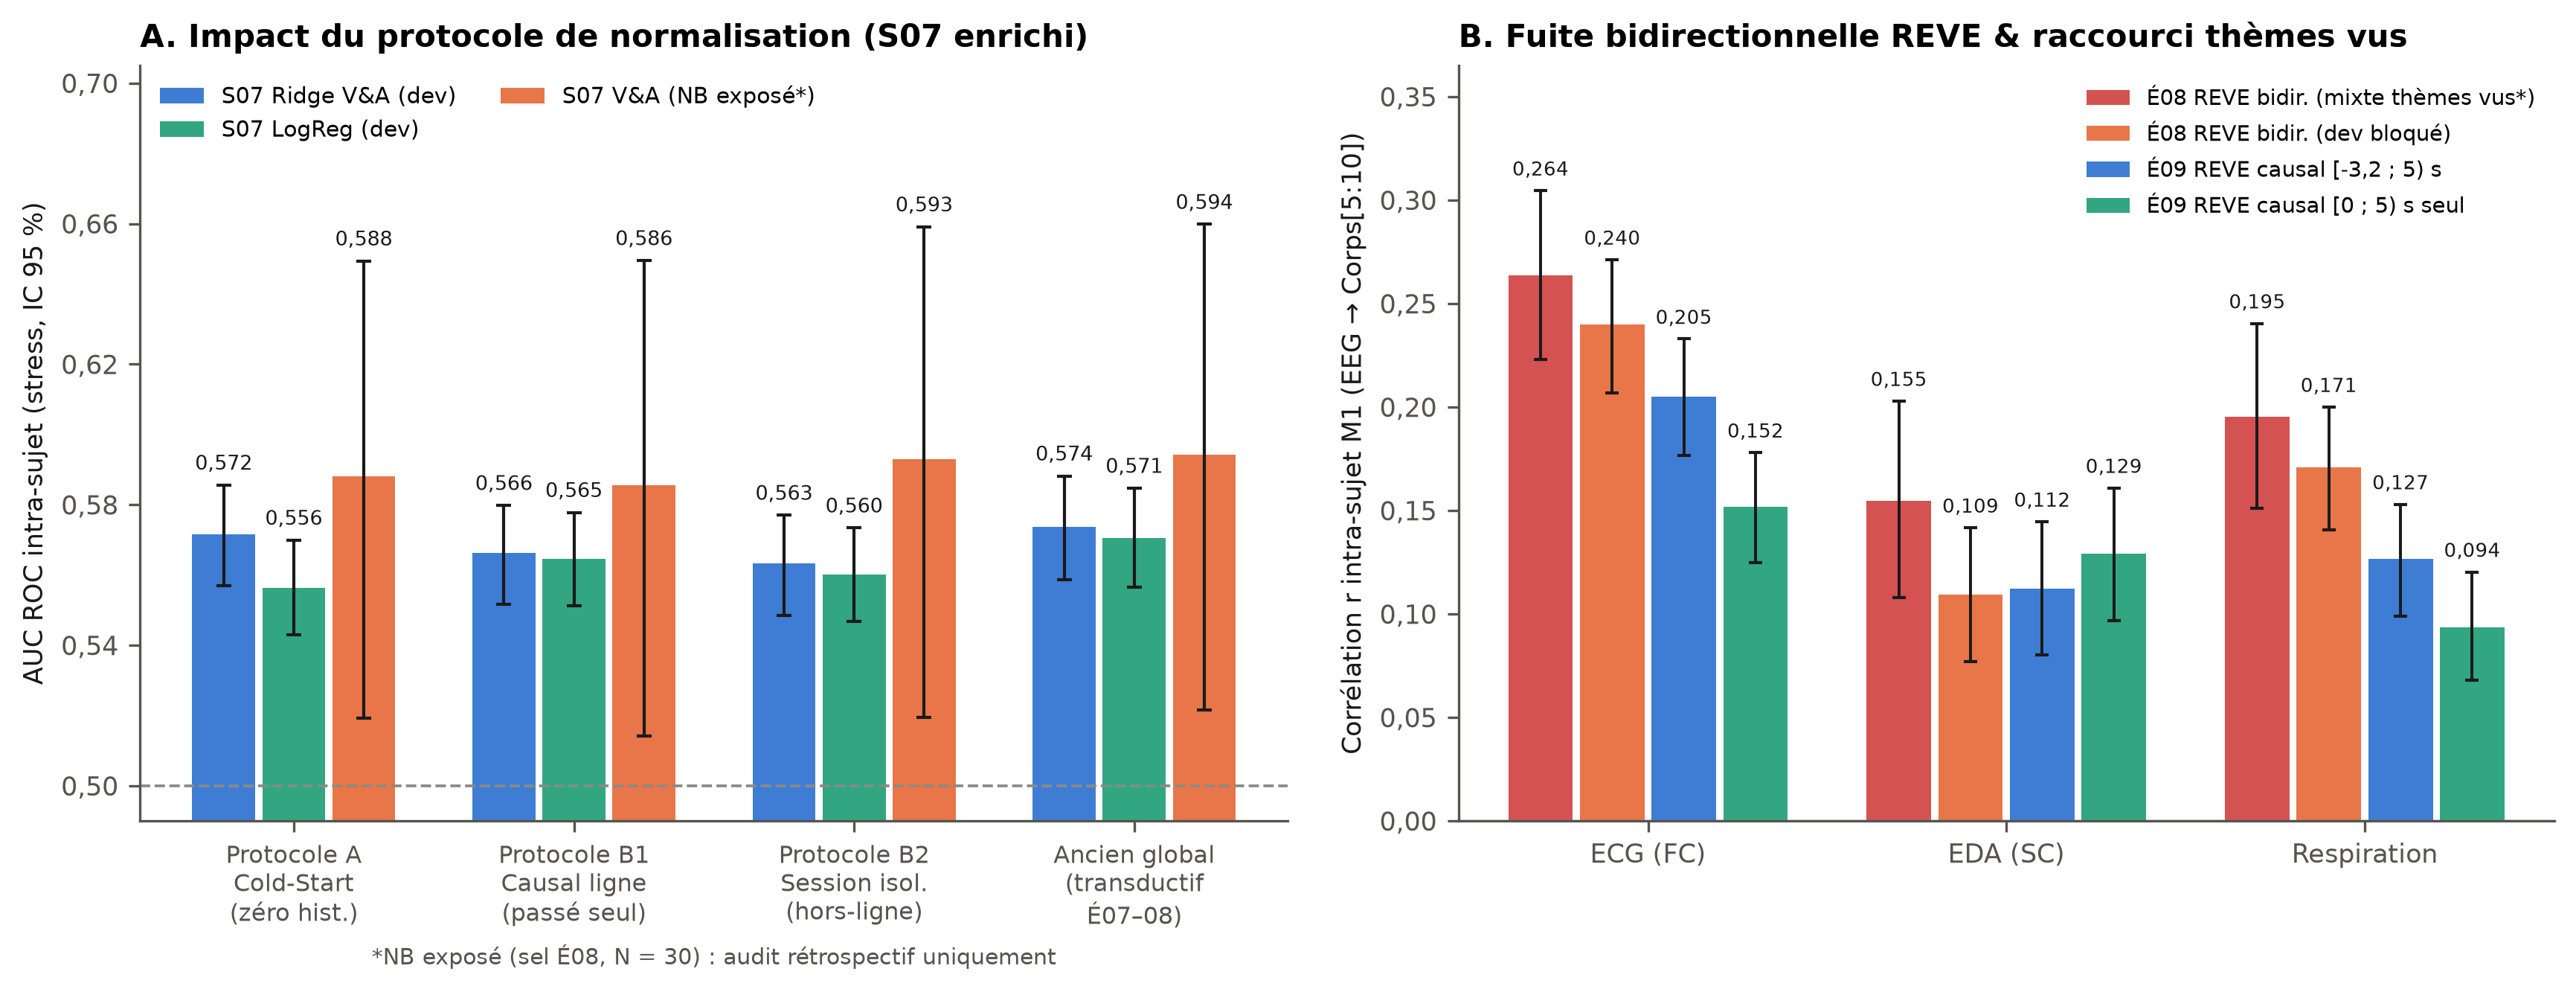
\includegraphics[width=\linewidth]{fig1_audit_fr.png}
\caption{\textbf{Audit quantitatif des Études 07--08.} \textbf{A.} Impact du protocole de normalisation sur \texttt{S07 enrichi} en \texttt{dev} ($3\times 3$) et sur le split exposé \texttt{test\_new\_both} ($N = 30$, audit rétrospectif uniquement). \textbf{B.} Inflation de la corrélation \texttt{M1} ($\text{EEG}\to\text{Corps}[5 ; 10)$~s) due à l'attention bidirectionnelle sur 13~s et aux 77\,\% de thèmes déjà vus dans l'Étude~08, comparée au mur causal strict à $t = 5{,}000$~s de l'Étude~09.}
\label{fig:audit}
\end{figure}

L'audit quantitatif (figure~\ref{fig:audit} et tableau~\ref{tab:audit}) confirme l'ampleur des deux biais identifiés dans le code. Sur le décodage de stress (\texttt{S07 enrichi}), la normalisation transductive globale (\texttt{legacy\_global}) gonflait la régression logistique directe sur \texttt{dev} de $+0{,}0141$ ($0{,}5564$ en Cold-Start $\to 0{,}5705$) et \texttt{Ridge V\&A} de $+0{,}0103$ par rapport à la session isolée ($0{,}5633 \to 0{,}5736$, $\bar{\rho} : 0{,}0880 \to 0{,}1019$). En Cold-Start strict, \texttt{Ridge V\&A} reste remarquablement stable ($0{,}5715$ [$0{,}5570 ; 0{,}5856$]), alors que la régression logistique directe bénéficie de l'historique causal en ligne B1 ($0{,}5564 \to 0{,}5646$).

L'impact de la fuite bidirectionnelle de \texttt{REVE-base} est encore plus marqué (figure~\ref{fig:audit}B). Sur le régime mixte de l'Étude~08 (77\,\% de thèmes vus), \texttt{REVE} bidirectionnel sur 13~s obtenait $r = 0{,}2638$ sur l'ECG, $0{,}1548$ sur l'EDA et $0{,}1954$ sur la respiration. En passant au découpage bloqué sujets~$\times$~thèmes (\texttt{dev}) et au mur causal dur à $t = 5{,}000$~s ($[-3{,}2 ; 5{,}0)$~s), ces corrélations \texttt{M1} chutent à \textbf{0,2050} ($-0{,}0588$) sur l'ECG, \textbf{0,1124} ($-0{,}0424$) sur l'EDA et \textbf{0,1265} ($-0{,}0689$) sur la respiration (et même $0{,}1518$ / $0{,}1290$ / $0{,}0937$ sur $[0 ; 5)$~s sans contexte pré-stimulus). Sur l'EDA en particulier, séparer les thèmes vus ($0{,}1662$) des thèmes inédits ($0{,}1048$) confirme un raccourci stimulus de $+0{,}0614$. De façon frappante, sous causalité stricte, l'EEG manuel (\texttt{M1\_hc\_eeg} : $0{,}2035$) égale désormais \texttt{REVE-base} ($0{,}1995$) sur l'ECG.

\begin{table}[t]
\centering\footnotesize
\begin{tabular}{@{}lrrrrrr@{}}
\toprule
Audit & Protocole / Représentation & \texttt{dev} V\&A & \texttt{dev} LogReg & ECG \texttt{M1} & EDA \texttt{M1} & Resp \texttt{M1}\\
\midrule
Normalisation & Protocole A : Cold-Start & 0,5715 & 0,5564 & — & — & —\\
(\texttt{S07 enrichi}) & Protocole B1 : Causal en ligne & 0,5662 & 0,5646 & — & — & —\\
 & Protocole B2 : Session isolée & 0,5633 & 0,5601 & — & — & —\\
 & Ancien global (transductif É07--08) & 0,5736 & 0,5705 & — & — & —\\
\midrule
Fuite \texttt{REVE} & É08 bidir.\ 13~s (mixte thèmes vus*) & — & — & 0,2638 & 0,1548 & 0,1954\\
(\texttt{M1} seul) & É08 bidir.\ 13~s (\texttt{dev} bloqué) & — & — & 0,2400 & 0,1094 & 0,1707\\
 & É09 causal strict $[-3{,}2 ; 5)$~s (\texttt{dev}) & — & — & \textbf{0,2050} & \textbf{0,1124} & \textbf{0,1265}\\
 & É09 causal strict $[0 ; 5)$~s seul (\texttt{dev}) & — & — & 0,1518 & 0,1290 & 0,0937\\
\bottomrule
\end{tabular}
\caption{Synthèse de l'audit des Études 07--08 (\texttt{audit\_forecast\_metrics.json}). *Split exposé de l'Étude~08 (audit rétrospectif uniquement).}
\label{tab:audit}
\end{table}

\subsection{Question principale : gain résiduel M2 contre M0 sur l'ECG, réfutation sur l'EDA et la respiration}

\begin{figure}[t]
\centering
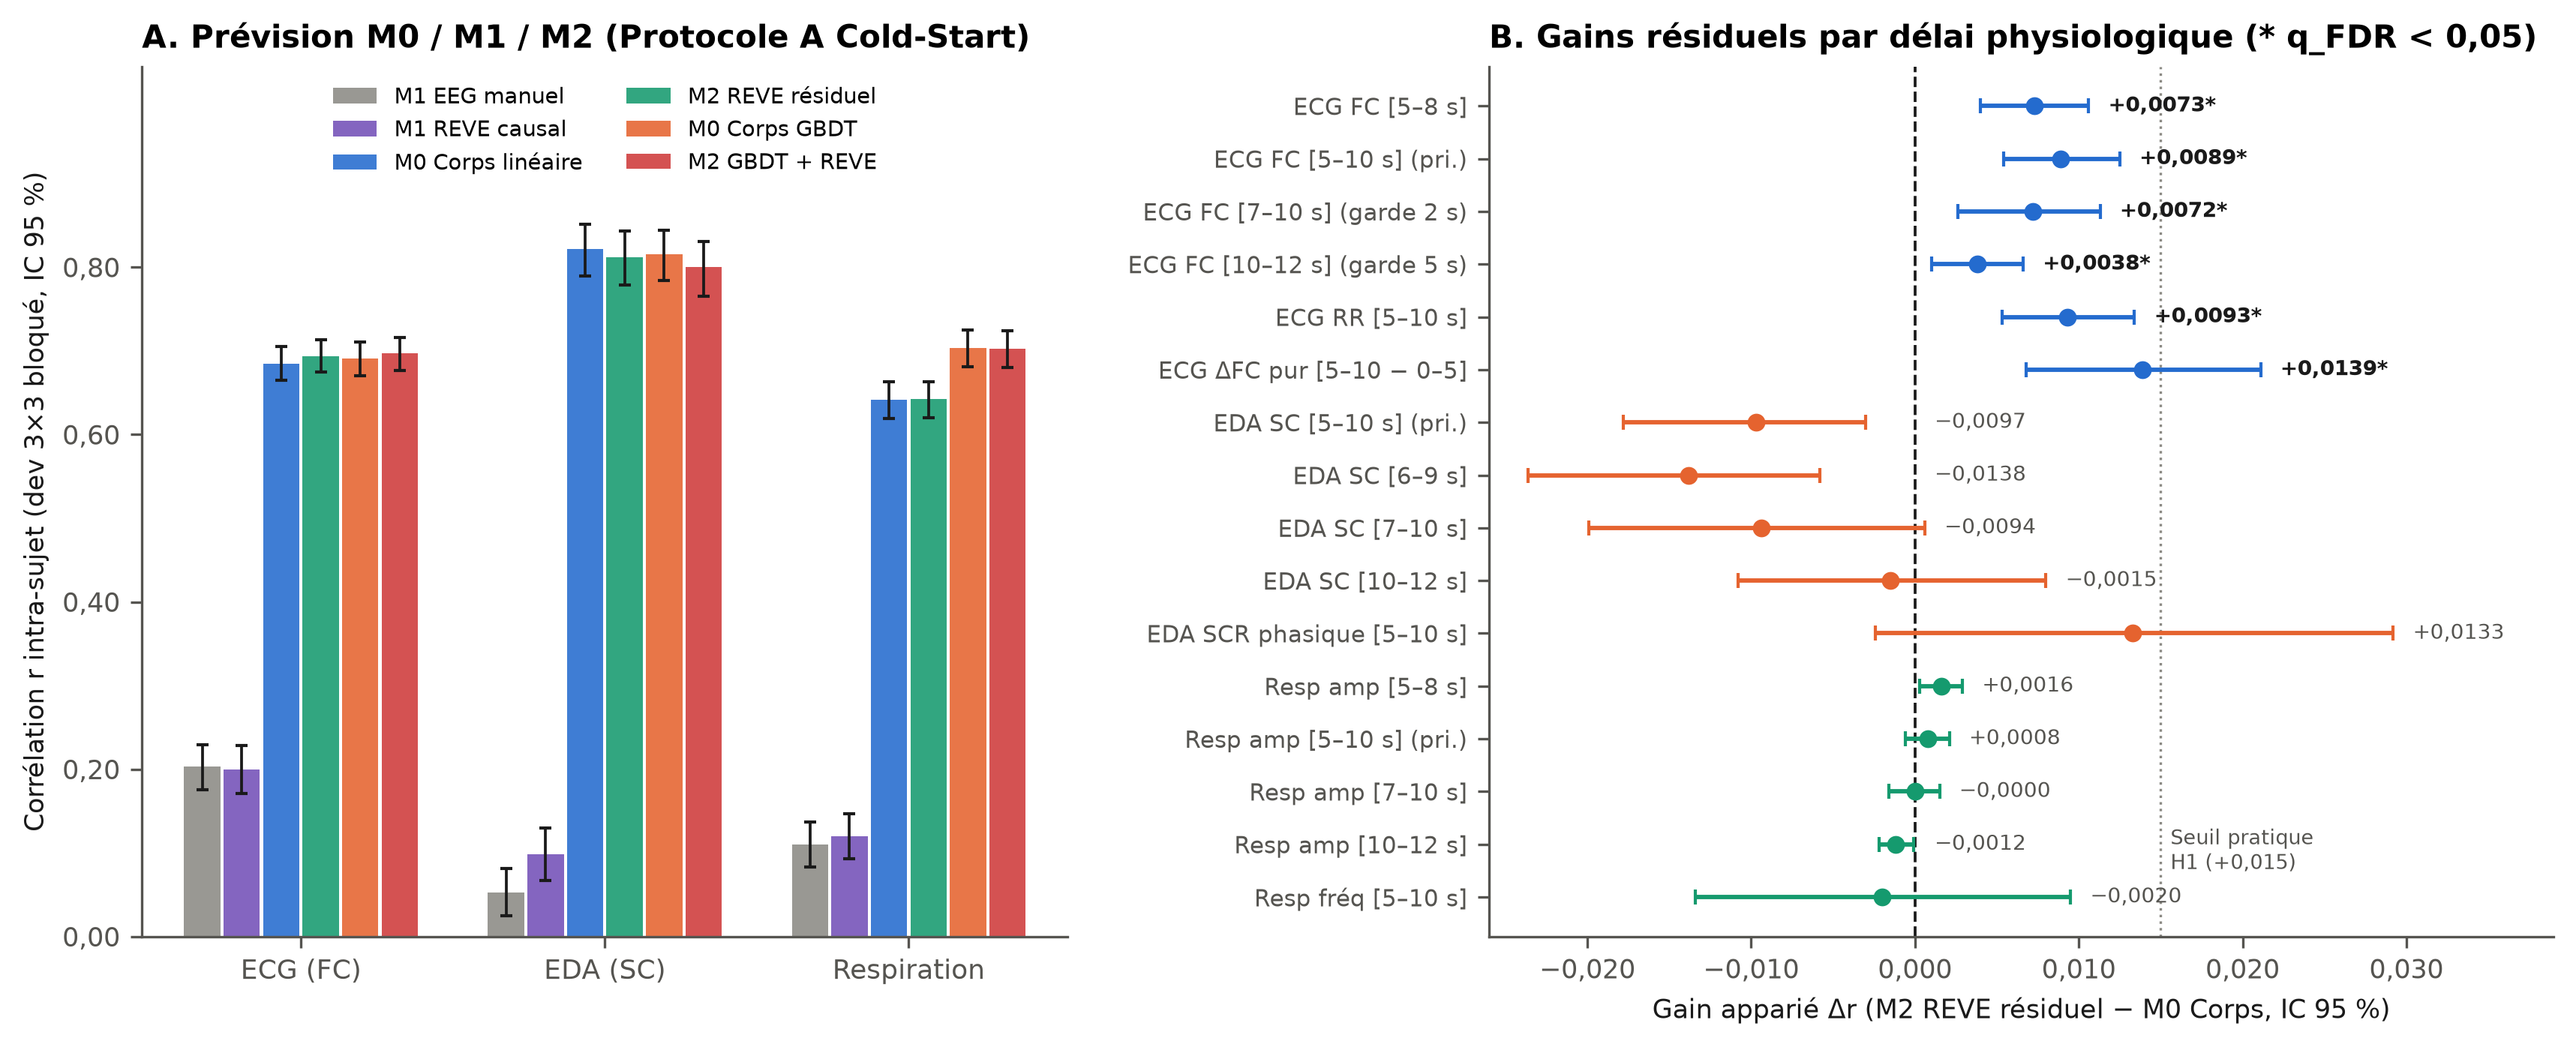
\includegraphics[width=\linewidth]{fig2_forecast_delays_fr.png}
\caption{\textbf{Question principale \texttt{M0 / M1 / M2} et délais physiologiques préspécifiés (\texttt{dev} $3\times 3$, Protocole~A Cold-Start).} \textbf{A.} Corrélation $r$ intra-sujet par organe et par famille de modèles (incluant le contrôle non linéaire \texttt{M0\_gbdt} / \texttt{M2\_gbdt\_reve}). \textbf{B.} Effets appariés $\Delta r$ (\texttt{M2\_reve\_resid $-$ M0\_linear}, IC~95\,\%) sur les 16 fenêtres et métriques principales (* indique $q_{\text{FDR}} < 0{,}05$ et borne inférieure $> 0$).}
\label{fig:forecast}
\end{figure}

La comparaison centrale \texttt{M0 / M1 / M2} (figure~\ref{fig:forecast} et tableau~\ref{tab:forecast}) établit une \textbf{dissociation organe nette} :

\paragraph{Dynamique cardiaque (ECG, $N = 224$) : signal incrémental réel, universel mais modeste.}
Le passé corporel seul (\texttt{M0\_linear}) explique déjà une grande part de la fréquence cardiaque future ($r = 0{,}6849$ [$0{,}6650 ; 0{,}7050$], $R^2_{\text{intra}} = 0{,}4530$). L'ajout de l'EEG précoce strictement causal améliore la prévision dans \textbf{toutes} les familles testées :
\begin{itemize}
\item \texttt{M2\_hc\_resid} (EEG manuel causal) : $\Delta r = +0{,}0071$ [$+0{,}0047 ; +0{,}0096$], 65,6\,\% améliorés, $q_{\text{FDR}} < 10^{-6}$.
\item \texttt{M2\_reve\_resid} (\texttt{REVE} gelé résiduel) : $\Delta r = +0{,}0089$ [$+0{,}0054 ; +0{,}0125$], médiane $+0{,}0063$ (IQR $-0{,}0041$ à $+0{,}0223$), $\Delta R^2_{\text{intra}} = +0{,}0106$, baisse RMSE $0{,}077$~bpm, 67,0\,\% améliorés ($q_{\text{FDR}} < 10^{-6}$).
\item \texttt{M2\_reve\_joint} (Ridge conjoint à double pénalité) : meilleur modèle linéaire ($r = 0{,}6959$), $\Delta r = +0{,}0110$ [$+0{,}0065 ; +0{,}0156$], médiane $+0{,}0101$, $\Delta R^2_{\text{intra}} = +0{,}0149$, réduction RMSE $0{,}086$~bpm, \textbf{71,4\,\%} des sujets améliorés ($q_{\text{FDR}} < 10^{-6}$).
\item \texttt{M2\_gbdt\_reve} contre \texttt{M0\_gbdt} : même au-dessus du modèle non linéaire sur le corps seul ($r = 0{,}6908$, $R^2_{\text{intra}} = 0{,}4664$), l'EEG conserve un gain significatif ($r = 0{,}6971$, $R^2_{\text{intra}} = 0{,}4746$, $\Delta r = +0{,}0063$ [$+0{,}0021 ; +0{,}0102$], $p = 7{,}3 \times 10^{-4}$).
\item Sensibilité $5\times 5$ et Protocoles~B : élargir la taille d'entraînement en CV~$5\times 5$ renforce le gain ($+0{,}0107$ résiduel, $+0{,}0120$ [$+0{,}0077 ; +0{,}0163$] conjoint) ; le gain reste hautement significatif sous B0 ($+0{,}0043$), B1 ($+0{,}0062$) et B2 ($+0{,}0047$, tous $p \le 3{,}4 \times 10^{-5}$).
\item Délais physiologiques et incrément pur : toutes les six cibles cardiaques passent $q_{\text{FDR}} < 0{,}02$ (figure~\ref{fig:forecast}B). Le gain est maximal sur l'incrément pur $\Delta\mathrm{FC}_{[5;10)-[0;5)}$ ($+0{,}0139$ résiduel, \textbf{$+0{,}0182$} [$+0{,}0086 ; +0{,}0276$] conjoint, franchissant le seuil pratique $+0{,}015$), confirmé sur l'intervalle RR ($+0{,}0093$, 72\,\% améliorés), et décroît biologiquement avec la distance temporelle : $+0{,}0073$ sur $[5 ; 8)$~s, $+0{,}0072$ ($+0{,}0089$ conjoint) sur $[7 ; 10)$~s (bande de garde stricte de 2~s) et $+0{,}0038$ [$+0{,}0010 ; +0{,}0066$] jusqu'à $[10 ; 12)$~s post-vidéo (garde de 5~s).
\end{itemize}
Toutefois, sur la cible primaire \texttt{tgt\_ecg\_hr\_chg\_5\_10}, le gain ($+0{,}0089$ à $+0{,}0110$) demeure inférieur au seuil d'effet pratique pré-enregistré de $+0{,}015$ : environ 97--98\,\% de la variance cardiaque prévisible sur $[5 ; 10)$~s est déjà capturée par l'état corporel précoce. De plus, l'adaptation LoRA en prévision (\texttt{M2\_reve\_lora} : $r = 0{,}6919$, $\Delta r = +0{,}0070$, 3 seeds $\text{ET} = 0{,}0013$) n'apporte aucun avantage sur la tête gelée ($-0{,}0001$ [$-0{,}0021 ; +0{,}0019$], $p = 0{,}385$) ni sur le modèle linéaire 0-GPU ($-0{,}0019$, $p = 0{,}139$).

\paragraph{Conductance cutanée (EDA, $N = 200$) et respiration ($N = 228$) : réfutation complète.}
Sur l'EDA, \texttt{M0\_linear} atteint déjà $r = 0{,}8218$ (médiane $R^2_{\text{intra}} = 0{,}8028$, intra-vidéo $0{,}9170$). Tous les modèles linéaires et GBDT intégrant l'EEG dégradent légèrement la prévision (\texttt{M2\_reve\_resid} $-0{,}0097$, \texttt{M2\_reve\_joint} $-0{,}0296$, \texttt{M2\_gbdt $-$ M0\_gbdt} $= -0{,}0155$) sur toutes les fenêtres ($5$--$10$, $6$--$9$, $7$--$10$, $10$--$12$~s). La légère amélioration de \texttt{M2\_reve\_lora} ($+0{,}0027$ [$0{,}0000 ; +0{,}0053$]) provient de la perte Smooth-L1 robuste aux valeurs extrêmes plutôt que de LoRA (\texttt{lora $-$ frozen\_head} $= +0{,}0015$, $p = 0{,}392$). Seul le nombre de nouveaux pics phasiques \texttt{SCR} ($[5 ; 10)$~s) montre une tendance positive non significative ($+0{,}0133$ [$-0{,}0024 ; +0{,}0292$], $q_{\text{FDR}} = 0{,}113$).

Sur la respiration, les modèles linéaires \texttt{M2} sont strictement nuls sur toutes les fenêtres ($+0{,}0008$ [$-0{,}0006 ; +0{,}0021$], $q = 0{,}346$). Fait méthodologique remarquable : la tête neuronale \texttt{M2\_reve\_frozen\_head} affichait un gain apparent de $+0{,}0096$ ($0{,}6417 \to 0{,}6514$) sur \texttt{M0\_linear}, mais le contrôle \texttt{M0\_gbdt} seul (sans EEG) atteint \textbf{0,7036} ($+0{,}0618$ au-dessus du linéaire, 83,8\,\% améliorés) et \texttt{M2\_gbdt\_reve} vaut \textbf{0,7028} ($\Delta r = -0{,}0008$ [$-0{,}0028 ; +0{,}0013$], $p = 0{,}453$). Le gain apparent de la tête neuronale provenait donc intégralement de la non-linéarité autorégressive du corps, et non de l'EEG.

\begin{table}[t]
\centering\scriptsize\setlength{\tabcolsep}{4pt}
\begin{tabular}{@{}llrrrrr@{}}
\toprule
Cible ($[5 ; 10)$~s) & Modèle & $r$ [IC 95\,\%] & $R^2_{\text{intra}}$ (méd.) & $\Delta r$ vs réf.\ [IC 95\,\%] & \% amél. & $p$ / $q_{\text{FDR}}$\\
\midrule
ECG FC ($N=224$) & \texttt{M0\_linear} & 0,6849 [0,665 ; 0,705] & 0,453 (0,447) & — & — & —\\
 & \texttt{M1\_reve} / \texttt{M1\_hc} & 0,1995 / 0,2035 & 0,009 / 0,026 & $-0{,}4855$ / $-0{,}4815$ & 3,1\,\% & $<10^{-6}$\\
 & \texttt{M2\_hc\_resid} & 0,6920 [0,672 ; 0,712] & 0,461 (0,456) & $+0{,}0071$ [$+0{,}005 ; +0{,}010$] & 65,6\,\% & $<10^{-6}$\\
 & \texttt{M2\_reve\_resid} & 0,6938 [0,675 ; 0,714] & 0,464 (0,463) & $\mathbf{+0{,}0089}$ [$+0{,}005 ; +0{,}013$] & 67,0\,\% & $<10^{-6}$\\
 & \texttt{M2\_reve\_joint} & \textbf{0,6959} [0,677 ; 0,716] & \textbf{0,468} (0,467) & $\mathbf{+0{,}0110}$ [$+0{,}007 ; +0{,}016$] & \textbf{71,4\,\%} & $<10^{-6}$\\
 & \texttt{M2\_reve\_lora} (3 seeds) & 0,6919 [0,673 ; 0,712] & 0,462 & $+0{,}0070$ [$+0{,}005 ; +0{,}010$] & 67,4\,\% & $<10^{-6}$\\
 & \texttt{M0\_gbdt} $\to$ \texttt{M2\_gbdt} & 0,6908 $\to$ \textbf{0,6971} & 0,466 $\to$ \textbf{0,475} & $\mathbf{+0{,}0063}$ [$+0{,}002 ; +0{,}010$] & 57,6\,\% & $7{,}3\times 10^{-4}$\\
\midrule
EDA SC ($N=200$) & \texttt{M0\_linear} & \textbf{0,8218} [0,789 ; 0,851] & (méd.\ 0,803) & — & — & —\\
 & \texttt{M2\_reve\_resid} / \texttt{joint} & 0,8121 / 0,7922 & (méd.\ 0,798) & $-0{,}0097$ / $-0{,}0296$ & 45,0\,\% & 0,016\\
 & \texttt{M0\_gbdt} $\to$ \texttt{M2\_gbdt} & 0,8158 $\to$ 0,8002 & (méd.\ 0,775) & $-0{,}0155$ [$-0{,}026 ; -0{,}007$] & 47,5\,\% & 0,104\\
\midrule
Resp ($N=228$) & \texttt{M0\_linear} & 0,6417 [0,619 ; 0,663] & 0,290 (0,407) & — & — & —\\
 & \texttt{M2\_reve\_resid} / \texttt{joint} & 0,6425 / 0,6428 & 0,290 (0,410) & $+0{,}0008$ [$-0{,}001 ; +0{,}002$] & 52,6\,\% & 0,289\\
 & \texttt{M0\_gbdt} $\to$ \texttt{M2\_gbdt} & \textbf{0,7036} $\to$ 0,7028 & \textbf{0,467} $\to$ 0,469 & $-0{,}0008$ [$-0{,}003 ; +0{,}001$] & 46,9\,\% & 0,453\\
\bottomrule
\end{tabular}
\caption{Comparaison principale \texttt{M0 / M1 / M2} sur \texttt{dev} ($3\times 3$ Cold-Start, \texttt{audit\_forecast\_metrics.json} et \texttt{study09\_lora\_forecast.json}).}
\label{tab:forecast}
\end{table}

\subsection{Contrôles d'artefacts, temporels, négatifs et preuve d'idiosyncrasie}

\begin{figure}[t]
\centering
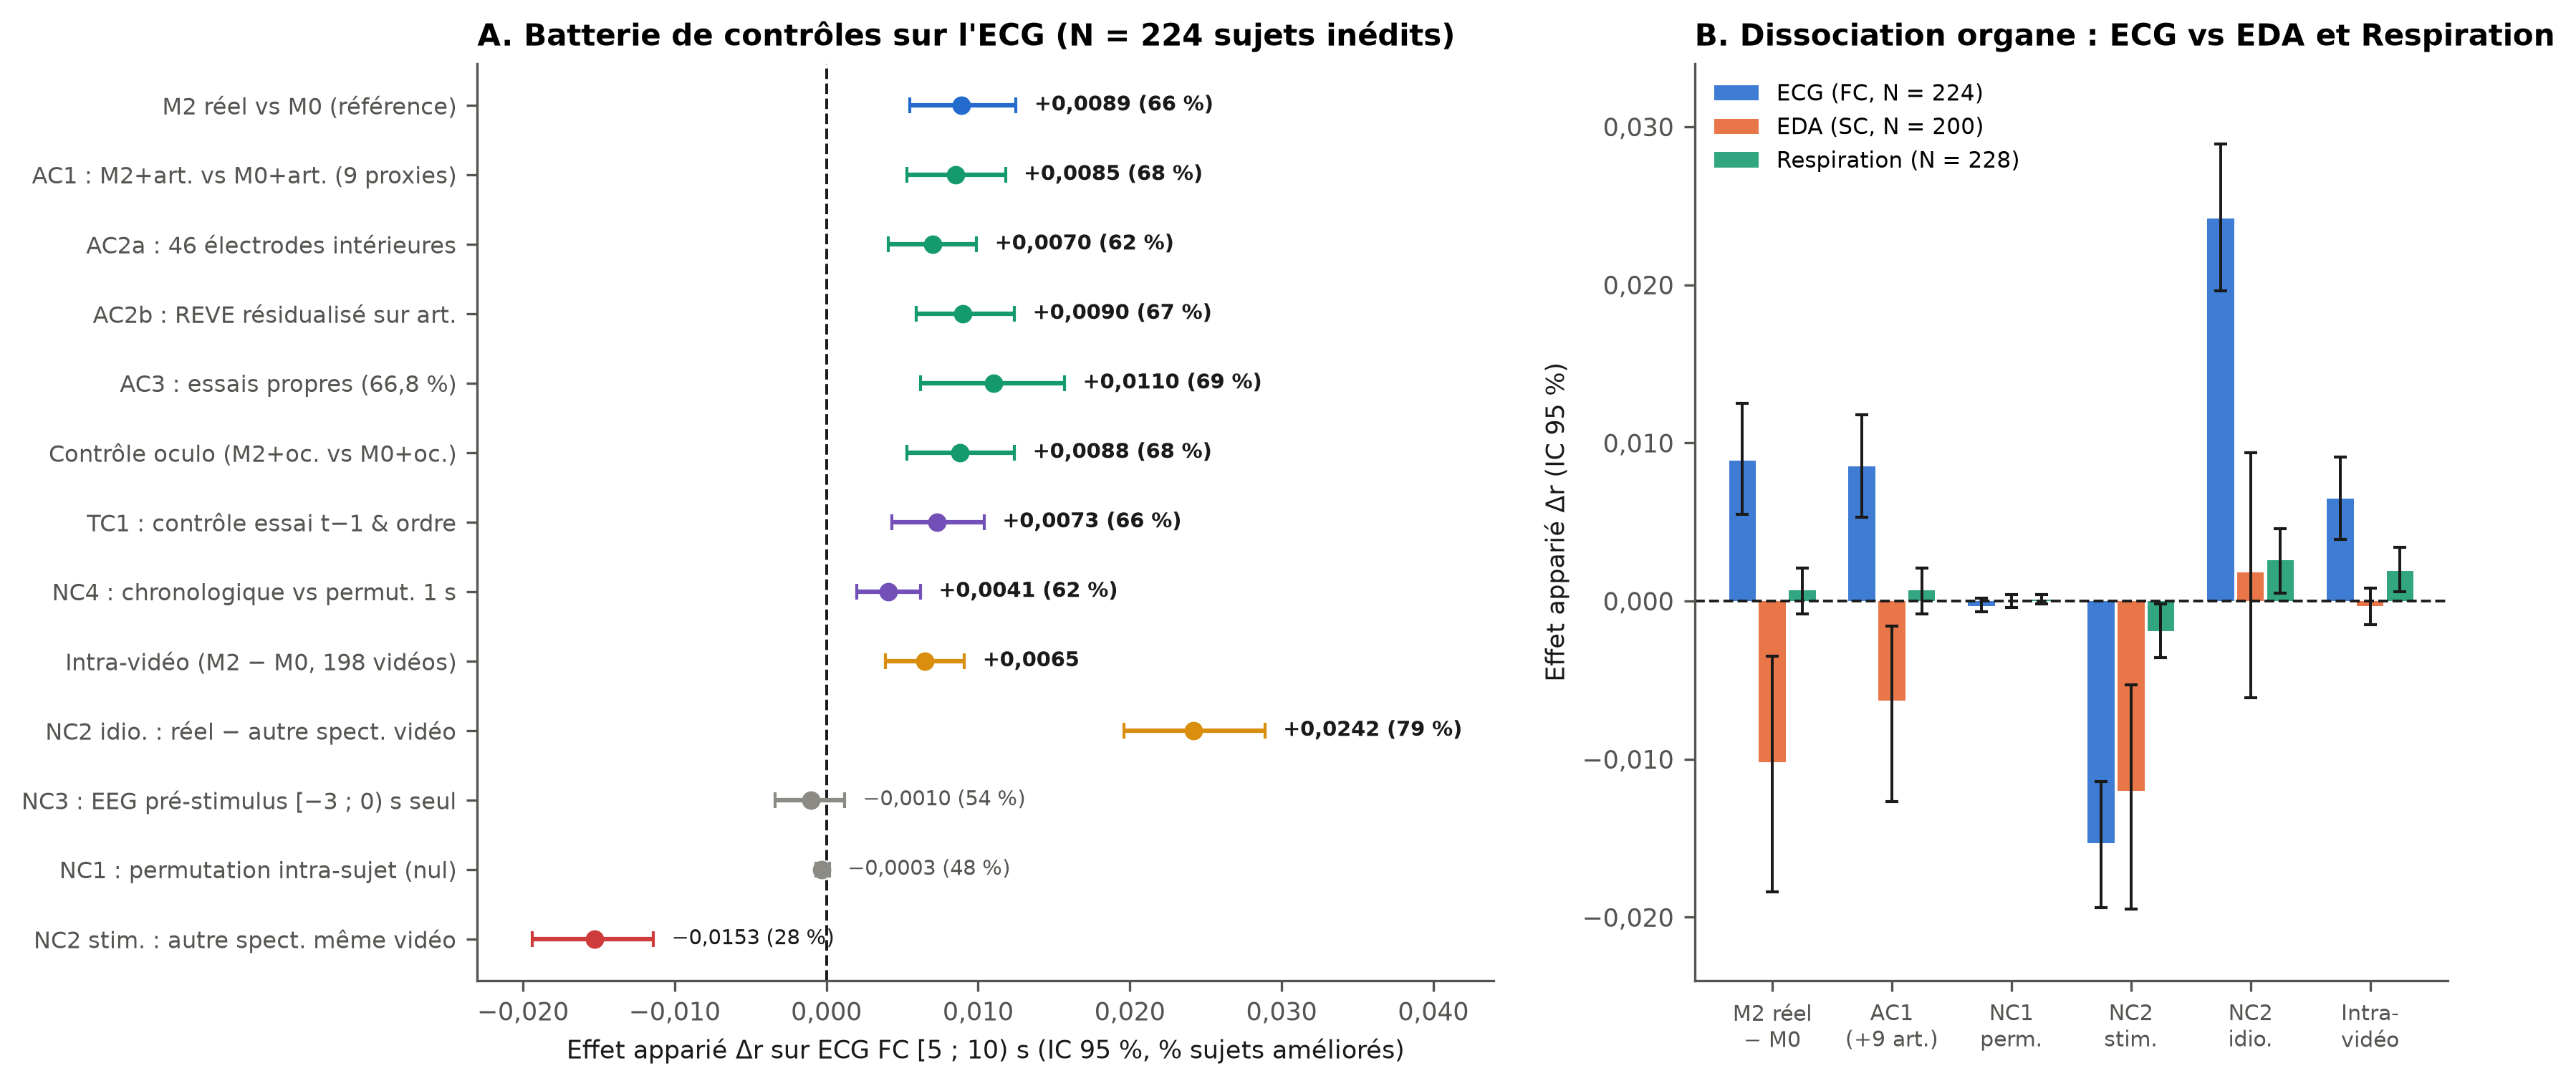
\includegraphics[width=\linewidth]{fig3_controls_fr.png}
\caption{\textbf{Batterie complète de contrôles (artefacts, dépendances temporelles, stimulus vs idiosyncrasie et contrôles négatifs).} \textbf{A.} Contrastes appariés $\Delta r$ (IC~95\,\%, pourcentage de sujets améliorés) sur l'ECG ($N = 224$). \textbf{B.} Comparaison directe entre ECG, EDA et respiration démontrant la spécificité cardiaque et la nature idiosyncrasique du signal.}
\label{fig:controls}
\end{figure}

La figure~\ref{fig:controls} tranche l'origine du signal cardiaque (\texttt{controls\_metrics.json}). Le détecteur de fuite \textbf{NC1} (permutation EEG intra-sujet) est exactement nul sur les trois organes ($-0{,}0003$ ECG, $+0{,}0000$ EDA, $+0{,}0001$ Resp). Sur l'ECG, le gain de référence ($+0{,}0089$) :
\begin{enumerate}
\item \textbf{n'est pas dû aux artefacts :} il demeure intact à 95,5\,\% avec les 9 covariables d'artefacts dans \texttt{M0} et \texttt{M2} (\textbf{AC1} : $+0{,}0085$, 67,9\,\%), à 78,7\,\% sur les 46 électrodes intérieures sans bordure (\textbf{AC2a} : $+0{,}0070$, $p = 2\times 10^{-6}$), à 101\,\% après résidualisation linéaire des artefacts (\textbf{AC2b} : $+0{,}0090$), à 99\,\% après ajout des 6 variables oculométriques ($+0{,}0088$), et \textbf{augmente sur les essais propres} (\textbf{AC3} : $+0{,}0110$ [$+0{,}0062 ; +0{,}0157$], 69,1\,\% améliorés) ;
\item \textbf{n'est pas un héritage de l'essai précédent ni du pré-stimulus :} il résiste à 82\,\% au contrôle de l'essai $t-1$ et de l'ordre (\textbf{TC1} : $+0{,}0073$, $p < 10^{-6}$) et s'annule totalement lorsque seul l'EEG pré-stimulus $[-3 ; 0)$~s est fourni (\textbf{NC3} : $-0{,}0010$ [$-0{,}0034 ; +0{,}0012$], $p = 0{,}877$) ;
\item \textbf{dépend de l'ordre chronologique dans $[0 ; 5)$~s :} permuter les cinq tranches de 1~s ramène \texttt{M2\_early5} ($0{,}6888$) exactement au niveau de \texttt{M0} ($0{,}6847$ vs $0{,}6849$ ; \textbf{NC4} chronologique $-$ permuté $= +0{,}0041$ [$+0{,}0020 ; +0{,}0062$], $p = 10^{-5}$) ;
\item \textbf{est strictement idiosyncrasique (non médié par le stimulus) :} dans \textbf{NC2}, remplacer l'EEG du spectateur par celui d'un autre participant regardant \emph{exactement la même vidéo inédite} dégrade la prédiction sous \texttt{M0} ($-0{,}0153$ [$-0{,}0194 ; -0{,}0114$]), donnant un contraste idiosyncrasique réel $-$ autre spectateur de \textbf{$+0{,}0242$} [$+0{,}0196 ; +0{,}0289$] (79,0\,\% améliorés, $\Delta R^2_{\text{intra}} = +0{,}0344$, $p < 10^{-6}$). Évalué strictement à vidéo fixe sur 198 clips, le gain intra-vidéo \texttt{M2 $-$ M0} vaut \textbf{$+0{,}0065$} [$+0{,}0039 ; +0{,}0091$].
\end{enumerate}

\subsection{REVE-base gelé contre LoRA multitâche, ranking intra-sujet et factorisation Trait/État}

\begin{figure}[t]
\centering
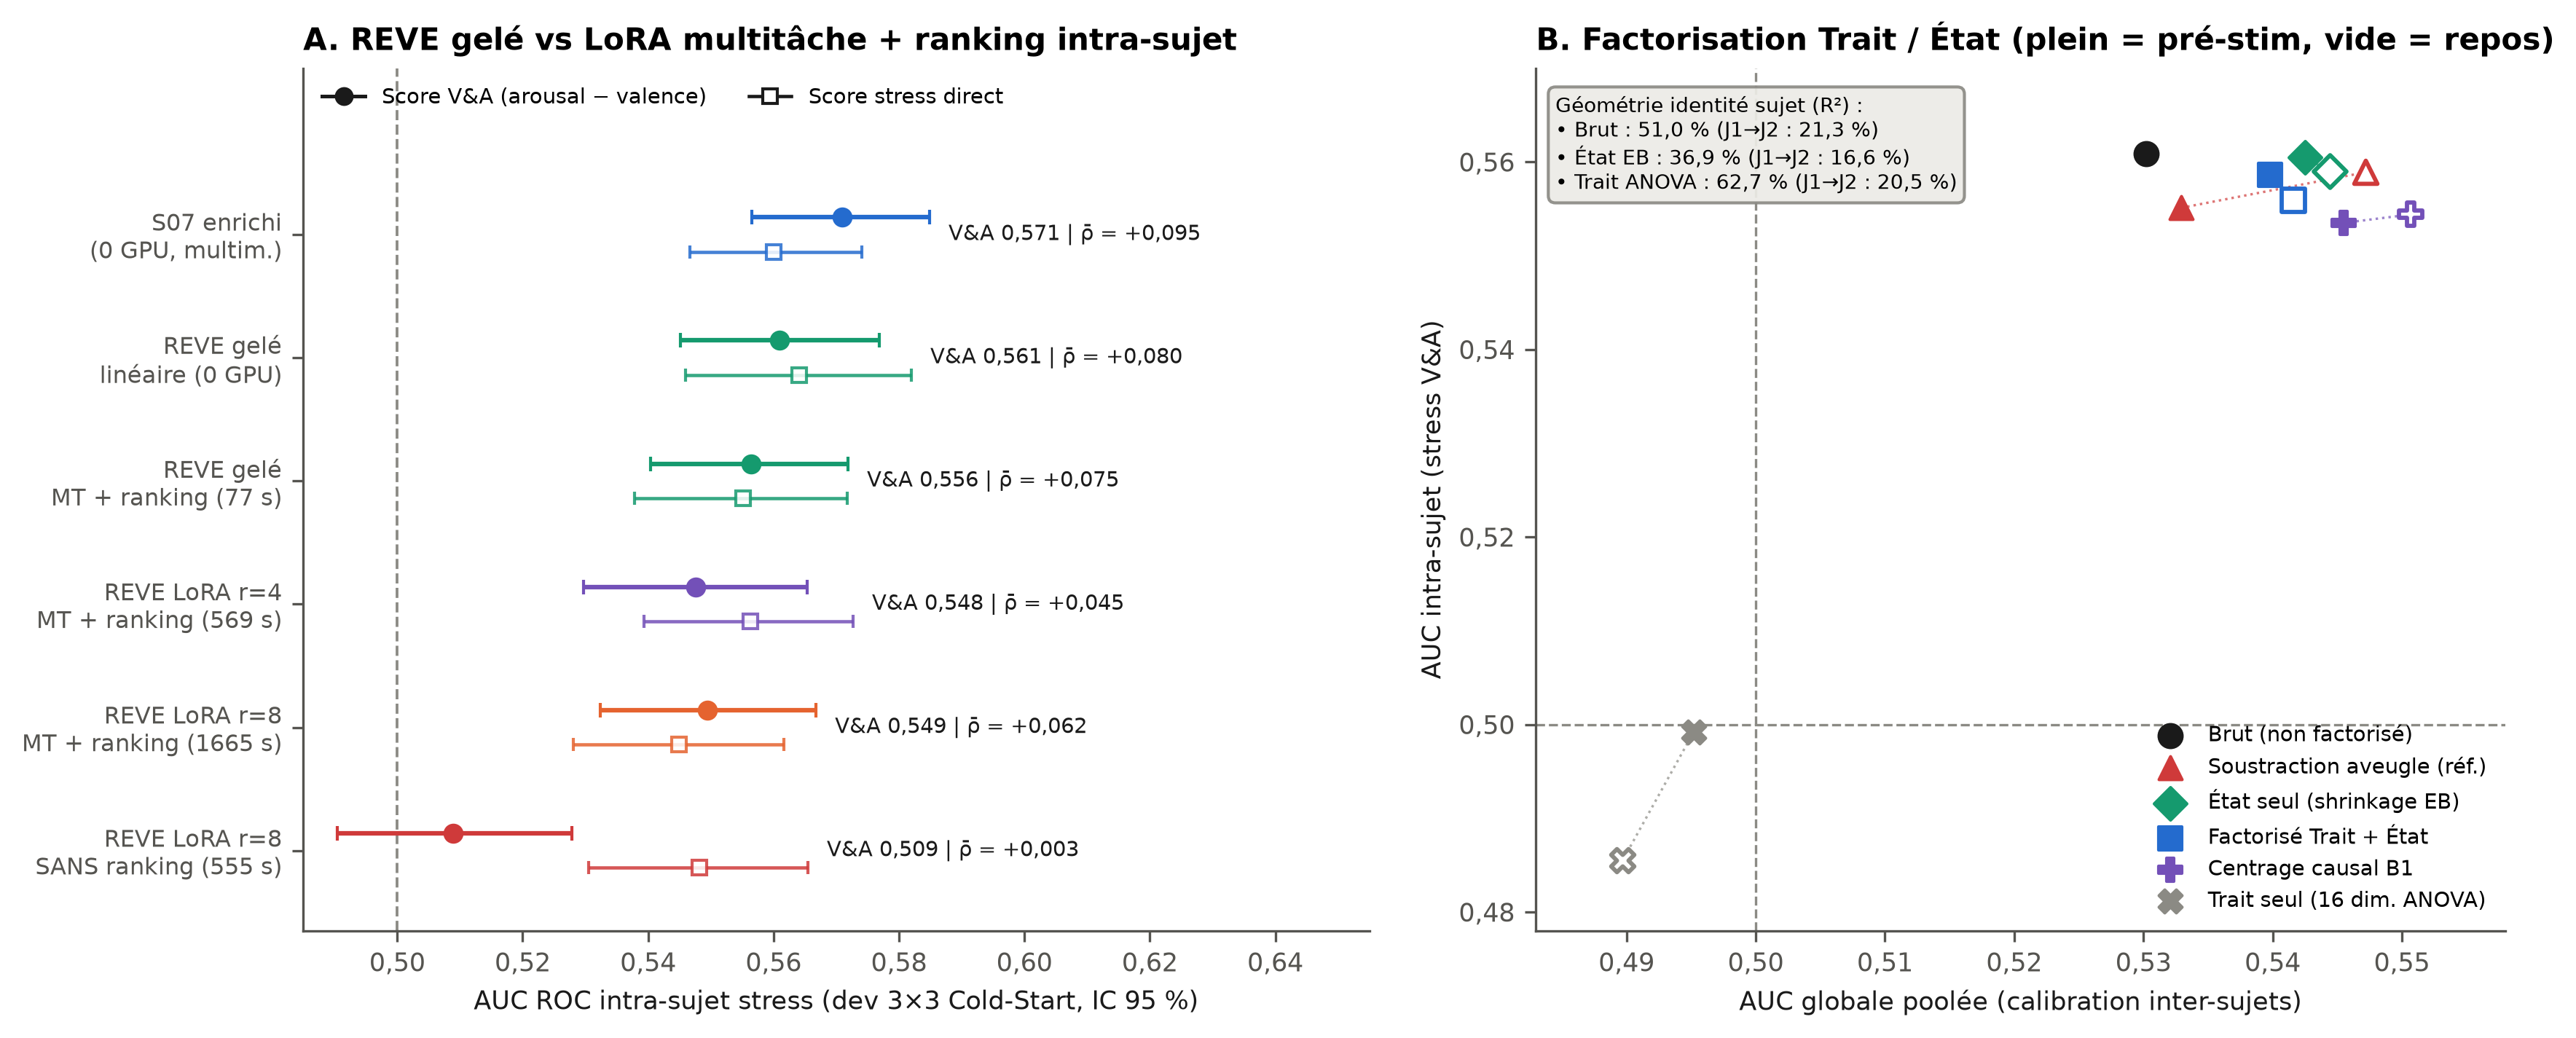
\includegraphics[width=\linewidth]{fig4_lora_trait_state_fr.png}
\caption{\textbf{Objectif secondaire (H2) et factorisation Trait/État (H3) sur \texttt{dev} ($3\times 3$ Cold-Start).} \textbf{A.} AUC stress (V\&A et direct) et corrélation affect $\bar{\rho}$ pour les modèles gelés vs LoRA : nul effet de LoRA pour 21,7$\times$ plus de calcul GPU, mais effondrement massif sans la perte de ranking intra-sujet. \textbf{B.} Compromis AUC intra-sujet contre AUC poolée globale et géométrie d'identité sujet ($R^2$ et identification inter-jours J1$\to$J2).}
\label{fig:lora_ts}
\end{figure}

Sur l'objectif secondaire de décodage du stress et de l'affect (figure~\ref{fig:lora_ts}A, \texttt{study09\_\allowbreak lora\_mt.json} et \texttt{secondary\_\allowbreak metrics.json}), deux constats nets s'imposent :
\begin{itemize}
\item \textbf{H2 réfutée pour LoRA :} en Cold-Start, la probe linéaire gelée sur \texttt{REVE-base} (0~s d'entraînement GPU) obtient une AUC stress V\&A de \textbf{0,5609} [$0{,}5451 ; 0{,}5769$] (direct $0{,}5641$, $\bar{\rho} = +0{,}0795$), dépassant à la fois la tête neuronale gelée multitâche+ranking (\texttt{reve\_mt\_frozen\_rank} : $0{,}5564$, $\bar{\rho} = +0{,}0752$, 76,7~s GPU), LoRA $r = 8$ (\texttt{reve\_mt\_lora\_rank} : $0{,}5495$, $\bar{\rho} = +0{,}0625$, 1\,665,0~s GPU, gain apparié $-0{,}0069$ [$-0{,}0211 ; +0{,}0070$] contre la tête gelée et $-0{,}0114$ [$-0{,}0254 ; +0{,}0021$] contre la probe linéaire) et LoRA $r = 4$ ($0{,}5476$, direct $0{,}5563$). Le modèle multimodal linéaire \texttt{S07\_enriched} reste en tête ($0{,}5709$, $\bar{\rho} = +0{,}0953$, $+0{,}0214$ [$+0{,}0016 ; +0{,}0407$] au-dessus de LoRA EEG).
\item \textbf{Rôle décisif de la perte de ranking intra-sujet :} supprimer le terme de ranking (\texttt{reve\_mt\_lora\_norank}) fait s'effondrer l'AUC V\&A de $0{,}5495$ à \textbf{0,5089} [$0{,}4904 ; 0{,}5279$] (perte appariée $-0{,}0406$ [$-0{,}0544 ; -0{,}0266$] face à LoRA+ranking et $-0{,}0475$ face à gelé+ranking) et réduit $\bar{\rho}$ à $+0{,}0026$ (arousal $-0{,}0247$). Sans centrage par sujet en Cold-Start, le ranking par paires intra-sujet empêche le réseau de gaspiller sa capacité sur les décalages inter-individuels.
\end{itemize}

L'analyse de factorisation Trait/État (figure~\ref{fig:lora_ts}B) explique ce mécanisme géométriquement. Sur \texttt{dev}, la représentation brute \texttt{REVE vid10} contient \textbf{51,01\,\%} de variance d'identité sujet (identification intra-session top-1 de 50,95\,\%, inter-jours J1$\to$J2 de 21,27\,\% contre 0,83\,\% au hasard). Soustraire aveuglément le vecteur pré-stimulus (\texttt{blind\_ref\_sub}) dégrade le décodage d'état ($0{,}5609 \to 0{,}5551$, LogReg $0{,}5641 \to 0{,}5451$, $\bar{\rho} : 0{,}0795 \to 0{,}0713$). À l'inverse, notre résidualisation par \emph{shrinkage} bayésien empirique (\texttt{state\_only\_shrinkage}) réduit $R^2_{\text{sujet}}$ à \textbf{36,94\,\%} (J1$\to$J2 $16{,}58\,\%$) tout en préservant intégralement l'AUC intra-sujet (\textbf{0,5605}), en élevant $\bar{\rho}$ à \textbf{+0,0822} et en améliorant nettement la calibration inter-sujets (AUC poolée $0{,}5302 \to 0{,}5425$, Brier $0{,}2489 \to 0{,}2479$ ; jusqu'à Brier $0{,}2471$ avec référence de repos B0). En revanche, le sous-espace trait ANOVA à 16 dimensions concentre $R^2_{\text{sujet}}$ à \textbf{62,68\,\%} (J1$\to$J2 $20{,}51\,\%$) mais n'encode pas la sensibilité subjective-trait au stress (\texttt{trait\_only} : AUC $0{,}4992$, $\rho_{\text{trait}} = -0{,}113$, réfutant le volet trait de H3).

\subsection{Audit oculométrique (508 enregistrements) et stacking conditionnel (H4--H5)}

\begin{figure}[t]
\centering
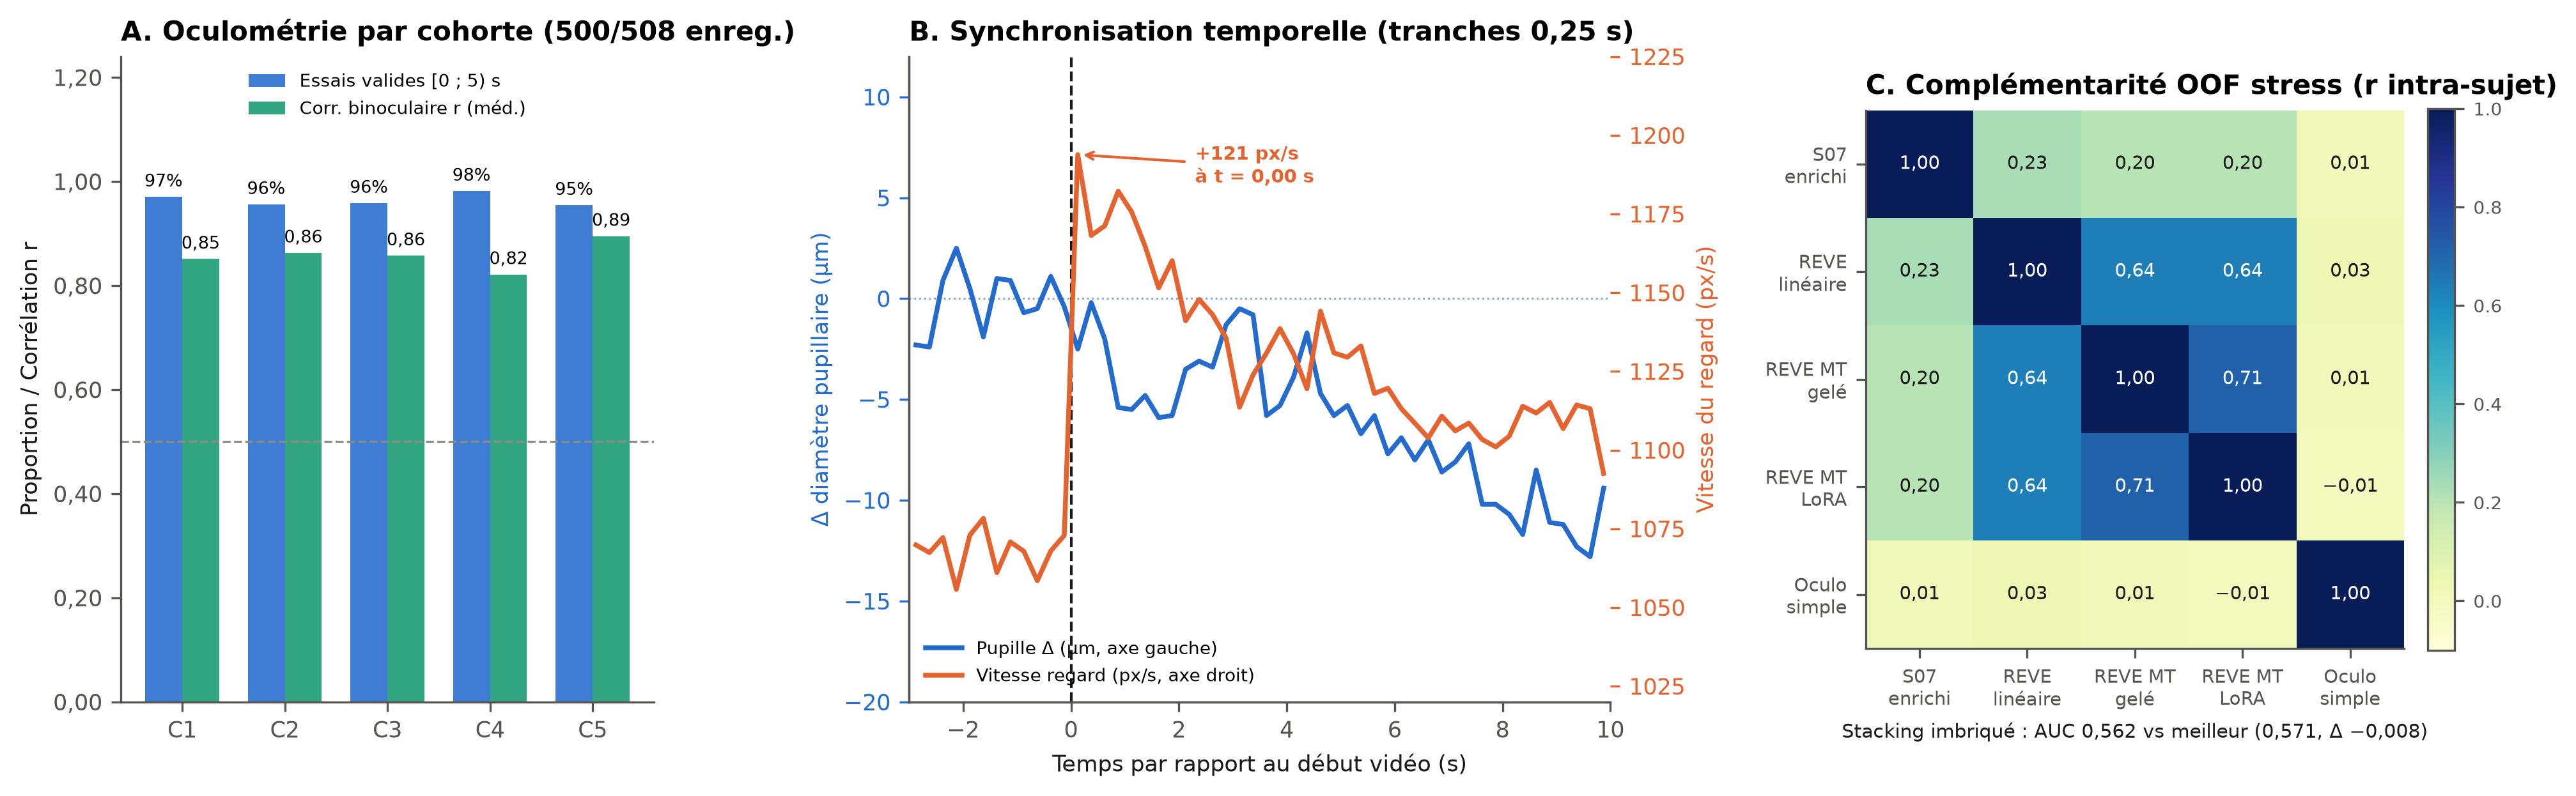
\includegraphics[width=\linewidth]{fig5_oculo_stacking_fr.png}
\caption{\textbf{Audit oculométrique complet (H4) et complémentarité / stacking OOF (H5).} \textbf{A.} Couverture valide $[0 ; 5)$~s et corrélation binoculaire gauche--droite médiane par cohorte (500/508 enregistrements). \textbf{B.} Courbes évoquées par tranches de 0,25~s : réponse pupillaire moyenne globale plate (échec de la porte stricte H4) contre décrochage instantané de la vitesse du regard à $t = 0{,}00$~s ($+121$~px/s). \textbf{C.} Matrice de corrélation OOF intra-sujet en stress et verdict du stacking imbriqué.}
\label{fig:oculo_stack}
\end{figure}

L'audit des 508 enregistrements (figure~\ref{fig:oculo_stack}A--B, \texttt{study09\_extract\_audit.json}) révèle un constat nuancé sur l'oculométrie, jusqu'ici écartée dans HABS : 500/508 enregistrements (98,4\,\%) contiennent des flux pupille/regard exploitables ($\approx 166$~Hz), avec \textbf{96,50\,\%} d'essais valides sur $[0 ; 5)$~s et une corrélation binoculaire gauche--droite médiane de \textbf{0,8519} ($0{,}821$ à $0{,}895$ selon les 5 cohortes). La porte pré-enregistrée stricte sur le réflexe pupillaire moyen $[0{,}25 ; 2{,}5)$~s échoue globalement ($-0{,}0040$~mm, $t = -1{,}259$, $p = 0{,}209$, probablement par compensation entre luminance hétérogène des vidéos et dilatation d'arousal ; seule la Cohorte~3 passe fortement : $-0{,}0301$~mm, $t = -5{,}65$, $p < 10^{-7}$). Néanmoins, la vitesse du regard exhibe un plateau plat à $1\,068{,}0 \pm 6{,}5$~px/s sur les 12 tranches pré-stimulus suivi d'un saut instantané à \textbf{1\,193,9~px/s} ($+121$~px/s, $+11{,}3\,\%$, $+19{,}4$~ET) dès la tranche $[0{,}00 ; 0{,}25)$~s, prouvant un alignement exact à $t = 0{,}00$~s. Les baselines exploratoires simples exécutées sur cette base restent cependant au hasard en détection de stress (Cold-Start V\&A $0{,}5058$ [$0{,}4918 ; 0{,}5196$], LogReg $0{,}4801$, $\bar{\rho} = -0{,}0007$ ; B1 causal $0{,}5024$) et confirment comme contrôle que le gain ECG \texttt{M2 $-$ M0} ne provient pas de l'oculométrie ($+0{,}0088$, 99\,\% intact).

Enfin, l'évaluation de la porte de complémentarité H5 (figure~\ref{fig:oculo_stack}C) conduit à une \textbf{abstention conforme sur l'EDA} (aucun modèle secondaire qualifié). Sur le stress, \texttt{REVE\_frozen\_linear} ($r_{\text{pred}} = 0{,}234$ avec \texttt{S07}, $r_{\text{partiel}} = +0{,}0763$ [$+0{,}0525 ; +0{,}0998$]) et \texttt{reve\_mt\_frozen\_rank} ($r_{\text{partiel}} = +0{,}0726$) franchissent la porte, tout comme \texttt{M1\_reve\_frozen} sur l'ECG ($r_{\text{partiel}} = +0{,}0629$) et la respiration ($+0{,}0421$). Pourtant, dans tous les cas, le méta-modèle OOF imbriqué échoue à battre le meilleur modèle unique (stress : $0{,}5625$ vs $0{,}5709$, $\Delta = -0{,}0084$ [$-0{,}0211 ; +0{,}0043$] ; ECG : $-0{,}0011$ [$-0{,}0033 ; +0{,}0010$] ; respiration : $-0{,}0057$ [$-0{,}0075 ; -0{,}0039$]), réfutant H5.

\section{Discussion, limites et portée méthodologique}

\begin{table}[t]
\centering\footnotesize
\begin{tabularx}{\linewidth}{@{}L{2.3cm} Y L{4.6cm}@{}}
\toprule
Hypothèse / Axe & Verdict vérifié & Chiffres clés (\texttt{dev} imbriqué)\\
\midrule
Audit 07--08 & Fuites transductives et bidirectionnelles quantifiées et corrigées. & LogReg $+0{,}0141$ ; \texttt{M1 REVE} $+0{,}059$ ECG, $+0{,}042$ EDA, $+0{,}069$ Resp.\\
H1 : ECG & Signal prédictif résiduel réel, idiosyncrasique, résistant aux artefacts, mais modeste ($< +0{,}015$ en primaire). & $\Delta r = +0{,}0089$ rés.\ / $+0{,}0110$ conj.\ (71,4\,\%), GBDT $+0{,}0063$, $\Delta\mathrm{FC}$ pur $+0{,}0182$, garde 2~s $+0{,}0089$, \texttt{NC2} idio.\ $+0{,}0242$.\\
H1 : EDA / Resp & Réfutée : aucune information EEG incrémentale au-delà du corps passé. & EDA $-0{,}0097$ (GBDT $-0{,}0155$) ; Resp $+0{,}0008$ (\texttt{M0\_gbdt} $0{,}7036$, \texttt{M2} $-0{,}0008$).\\
H2 : LoRA / Rank & LoRA réfuté (21,7$\times$ coût GPU, gain nul) ; ranking intra-sujet décisif. & LoRA $-0{,}0069$ vs gelé ; \texttt{rank $-$ norank} $= +0{,}0406$ ($0{,}5089 \to 0{,}5495$).\\
H3 : Trait/État & \emph{Shrinkage} EB préserve l'état et calibre mieux ; trait EEG $\not\to$ stress-trait. & État EB $0{,}5605$ (vs aveugle $0{,}5551$), $R^2_{\text{ID}}$ $51\,\% \to 37\,\%$, Brier $0{,}2479$ ; trait $\rho = -0{,}113$.\\
H4 : Oculométrie & Porte pupillaire stricte échouée ; alignement regard prouvé ; stress nul. & Couv.\ 96,5\,\%, $r_{\text{binoc}} = 0{,}852$, regard $+121$~px/s à $t = 0$~s ; stress $0{,}5058$.\\
H5 : Stacking & Réfutée (abstention EDA, aucun gain sur stress, ECG et respiration). & Stress $-0{,}0084$, ECG $-0{,}0011$, Resp $-0{,}0057$.\\
\bottomrule
\end{tabularx}
\caption{Synthèse des verdicts pré-enregistrés de l'Étude 09 (1,40~H100-h et 3,41~CPU-h reproductibles).}
\label{tab:verdicts}
\end{table}

\paragraph{Ce que démontre la dissociation cardiaque vs électrodermale et respiratoire.}
Le tableau~\ref{tab:verdicts} éclaire la physiologie du stress aigu bref à une échelle rarement atteinte (224--228 sujets inédits dans un protocole sans fuite). L'existence d'une information prédictive EEG précoce $\to$ fréquence cardiaque future, strictement idiosyncrasique (détruite si l'on substitue l'EEG d'un autre spectateur de la même vidéo), ordonnée dans le temps (\textbf{NC4}), persistante après 2 à 5~s de garde et insensible aux 9 proxies d'artefacts, à l'ablation des 16 électrodes de bordure et à l'oculométrie, est cohérente avec un couplage central--vagal rapide modulant la décélération cardiaque évaluative \cite{thayer2009,parkblanke2019}. En même temps, sa faible ampleur incrémentale ($\Delta r \approx +0{,}009$ à $+0{,}012$, $\Delta R^2_{\text{intra}} \approx 1{,}1$--$1{,}5\,\%$) et son absence sur la conductance cutanée et la respiration rappellent un fait quantitatif essentiel : sur des clips de 10~s, la trajectoire autonome future $[5 ; 10)$~s est déjà très fortement déterminée par l'état périphérique initial $[0 ; 5)$~s ($r = 0{,}685$--$0{,}822$).

\paragraph{Leçons méthodologiques pour les modèles fondation EEG.}
Trois enseignements directement transférables ressortent de nos expériences. Premièrement, l'usage de modèles fondation EEG bidirectionnels (\texttt{REVE}, \texttt{CBraMod}, \texttt{LaBraM}) pour des tâches prédictives temporelles impose un \textbf{mur causal matériel avant l'encodage} (et un test unitaire de non-invariance au futur), faute de quoi l'attention bidirectionnelle crée des corrélations illusoires. Deuxièmement, face à une baseline autorégressive forte, l'évaluation doit impérativement inclure un modèle non linéaire \texttt{M0\_gbdt} : sans lui, la tête neuronale sur la respiration aurait créé un faux positif de $+0{,}0096$. Troisièmement, en décodage affectif \emph{cold-start} sur un grand échantillon multi-sujets, l'adaptation LoRA sur-ajuste les 66 thèmes d'entraînement à coût GPU élevé, tandis que l'alignement de la fonction objectif (ranking intra-sujet) et le débruitage par \emph{shrinkage} bayésien empirique apportent des gains réels et interprétables.

\paragraph{Discipline épistémique, limites et reproductibilité.}
Nous maintenons une séparation stricte entre \emph{prédiction temporelle conditionnelle}, \emph{association} et \emph{causalité mécanistique} : un gain \texttt{M2 $-$ M0} contrôlé établit une prévisibilité incrémentale au sens de Granger, non une causalité efférente directe (un processus sous-cortical ou vasculaire non mesuré pouvant précéder simultanément l'EEG et la variation cardiaque). Nous ne revendiquons aucun plafond physiologique universel : nos conclusions valent conditionnellement à des clips passifs de 10~s, 62 électrodes de scalp et \texttt{REVE-base}. Enfin, l'ensemble du code (\texttt{decoding/\allowbreak study09\_*.py}), des tests unitaires (\texttt{tests/\allowbreak test\_study09\_*.py}), du protocole et journal d'exécution (\texttt{journal/\allowbreak 09\_eeg\_predictive\_physiology.md}), des six fichiers JSON agrégés (\texttt{docs/\allowbreak research/\allowbreak study09/\allowbreak results/}) et du script des figures (\texttt{docs/\allowbreak research/\allowbreak study09/\allowbreak make\_figures.py}) est versionné dans le dépôt, sans qu'aucune donnée individuelle ne quitte les serveurs HABS.

\begin{otherlanguage*}{english}
\begin{thebibliography}{99}\footnotesize\setlength{\itemsep}{1.2pt}
\bibitem{palomba2000} D. Palomba, M. Sarlo, A. Angrilli, A. Mini, L. Stegagno. Cardiac responses associated with affective processing of unpleasant film stimuli. Int. J. Psychophysiol. 36 (2000) 45--57.
\bibitem{hagenaars2014} M. A. Hagenaars, K. Roelofs, J. F. Stins. Human freezing in response to affective films. Anxiety, Stress, \& Coping 27 (2014) 27--37.
\bibitem{benedek2010} M. Benedek, C. Kaernbach. A continuous measure of phasic electrodermal activity. J. Neurosci. Methods 190 (2010) 80--91.
\bibitem{thayer2009} J. F. Thayer, R. D. Lane. Claude Bernard and the heart--brain connection: further elaboration of a model of neurovisceral integration. Neurosci. Biobehav. Rev. 33 (2009) 81--88.
\bibitem{parkblanke2019} H.-D. Park, O. Blanke. Heartbeat-evoked cortical responses: underlying mechanisms, functional roles, and methodological considerations. NeuroImage 197 (2019) 502--511.
\bibitem{giannakakis2015} G. Giannakakis, D. Grigoriadis, M. Tsiknakis. Detection of stress/anxiety state from EEG features during video watching. IEEE EMBC 2015, 6034--6037.
\bibitem{gerster2026} M. Gerster et al. Stimulus identity rather than emotion drives EEG classification on the FACED dataset. bioRxiv 2026, doi:10.64898/2026.06.12.731889.
\bibitem{varoquaux2018} G. Varoquaux. Cross-validation failure: small sample sizes lead to large error bars. NeuroImage 180 (2018) 68--77.
\bibitem{hu2022} E. J. Hu et al. LoRA: Low-Rank Adaptation of Large Language Models. ICLR 2022.
\bibitem{reve2025} J. O. El Ouahidi et al. REVE: A Foundation Model for EEG -- Adapting to Any Setup with Large-Scale Pretraining on 25,000 Subjects. arXiv:2510.21585 (2025).
\end{thebibliography}
\end{otherlanguage*}

\end{document}
